\section{Grundlagen}
\begin{frame}
    \frametitle{Feedforward Neural Networks \cite[164]{Goodfellow-et-al-2016}}

    \begin{itemize}
        \item Approximiert eine Funktion $ y = f(x; \theta) $ anhand der Gewichtungsvariablen $ \theta $
        \item Kann aus mehreren Layern bestehen die in einer Kettenstruktur ineinander gehen: $ f(x) = f^{(3)}(f^{(2)}(f^{(1)}(x))) $
        \item Durch die Minimierung einer Loss-Funktion wird $ \theta $ mathematisch optimiert und das Netzwerk trainiert
    \end{itemize}
\end{frame}

\begin{frame}
    \frametitle{Convolutions}

    \begin{itemize}
        \item Spezielle Art von Layer innerhalb eines Neuralen Netzwerks
        \item Eignet sich optische Features zu erlernen
        \item Tiefere Layer lernen komplexere Features innerhalb eines CNNs
    \end{itemize}
    
    \begin{figure}[H]
        \centering
        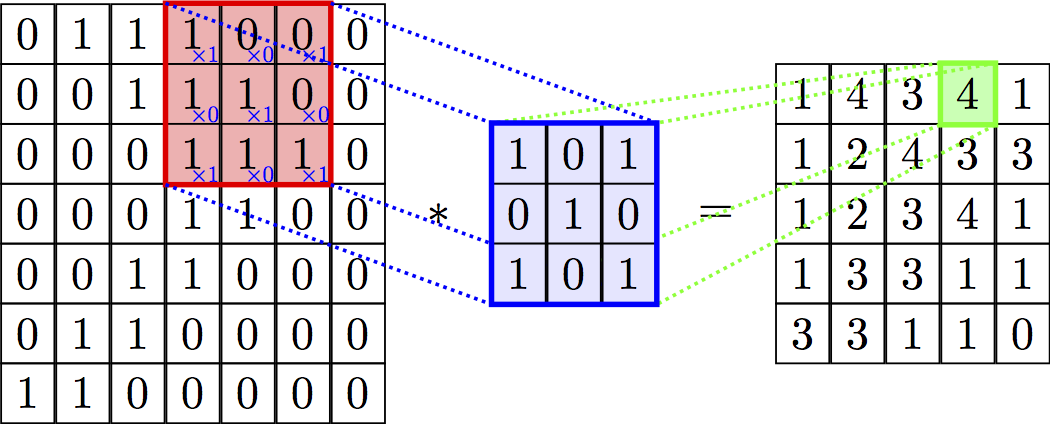
\includegraphics[width=0.75\textwidth]{resources/content/convolution_croped.png}
        \caption{Kernel der Convolution wird gelernt \cite{convolution_img}}
        \label{img:convolution}
    \end{figure}
\end{frame}


\begin{frame}
    \frametitle{VGG16 \cite{DBLP:journals/corr/SimonyanZ14a}}

    Auf dem ImageNet-Datensatz \cite{5206848} vortrainiertes Modell
    \begin{figure}[H]
        \centering
        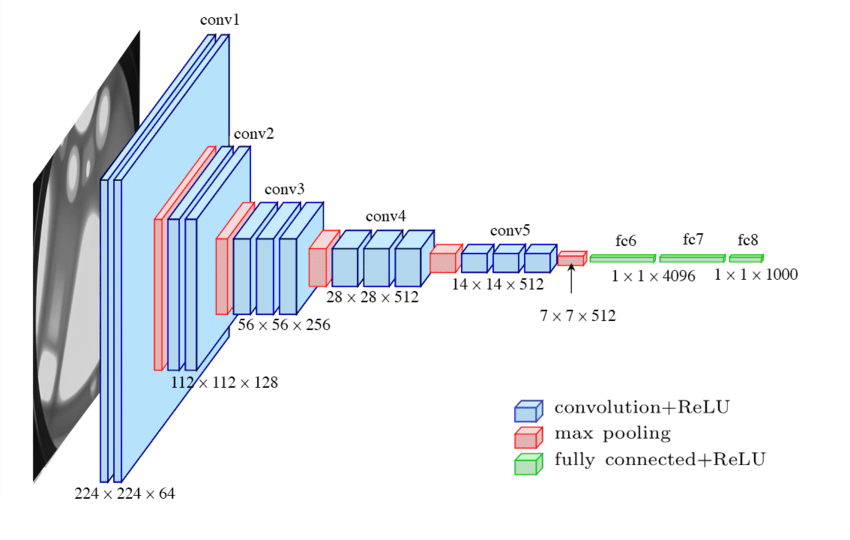
\includegraphics[width=0.75\textwidth]{resources/content/vgg16.png}
        \caption{Architektur des VGG16-Netzwerks \cite{vgg16_img}}
        \label{img:vgg16_img}
    \end{figure}

\end{frame}